\documentclass{article}

\usepackage{graphicx}
\usepackage{indentfirst}
\usepackage[a4paper, total={6in, 8in}]{geometry}
\usepackage{hyperref}
\usepackage{amsmath,amsfonts,amssymb}
\usepackage{fancyhdr}
\usepackage{xepersian}
\settextfont{B Nazanin}
\setlatintextfont{Times New Roman}


\renewcommand{\labelitemi}{$\bullet$}

\begin{document}


%title page%
\begin{titlepage}
	\begin{center}
		\textbf{ \Huge{به نام خدا}}	
		\vspace{0.2cm}
		
		
\includegraphics[width=0.4\textwidth]{sharif.png}\\
		\vspace{0.2cm}
		\textbf{ \Huge{آزمایش شماره 4}}\\
		\vspace{0.25cm}
		\textbf{ \Large{آز معماری - دکتر سربازی آزاد}}
		\vspace{0.2cm}
		
		
		\large \textbf{دانشکده مهندسی کامپیوتر}\\\vspace{0.1cm}
		\large   دانشگاه صنعتی شریف\\\vspace{0.2cm}
		\large   ﻧﯿﻢ‌سال اول ۰۰-۰۱ \\\vspace{0.10cm}
		\large{گروه:}\\
		\large{\href{mailto:a.h.hadian@gmail.com}{امیرحسین هادیان - ۹۷۱۰۲۶۰۹}}\\
		\large{\href{mailto:mofayezi.m@gmail.com}{محمدرضا مفیضی - ۹۸۱۰۶۰۵۹}}\\
		\large{\href{mailto:a.hatam008@gmail.com}{علی حاتمی تاجیک - ۹۸۱۰۱۳۸۵}}\\
	\end{center}
\end{titlepage}
%title page%

\newpage

%pages header
\pagestyle{fancy}
\fancyhf{}
\fancyfoot{}
\setlength{\headheight}{59pt}
\cfoot{\thepage}
\lhead{آزمایش شماره 4}
\rhead{
\includegraphics[width=0.1\textwidth]{sharif.png}\\
		دانشکده مهندسی کامپیوتر
}
\chead{آز معماری}
%pages header

\section{هدف}
در این آزمایش قصد داریم یک مبدل دهدهی به دودویی را طراحی و پیاده‌سازی کنیم. با فعال شدن سیگنال شروع مدار شروع به کار کرده و ورودی دهدهی را که یک عدد سه رقمی است به معادل دودویی آن تبدیل می‌کند و حاصل را در خروجی قرار می‌دهد و سیگنال پایان را فعال می‌کند.

\section{الگوریتم}
برای تبدیل یک عدد دهدهی \lr{r}رقمی به معادل دودویی به صورت زیر عمل می‌کنیم:
\begin{enumerate}
	\item عدد دهدهی ورودی را یک بیت به راست شیفت می‌دهیم.
	
	\item اگر با ارزشترین بیت رقم \lr{i}ام یک باشد از آن رقم 3 واحد کم می‌کنیم.
	
	\item مراحل اول و دوم را آنقدر تکرار می‌کنیم تا تمام ارقام دهدهی صفر شوند.
	
\end{enumerate}
 
در پایان بیت‌هایی که بوسیله شیفت به راست بیرون می‌آیند، عدد دودویی معادل عدد دهدهی ورودی را تشکیل می‌دهند.

\section{طراحی}
\subsection{\lr{ASM Chart}} 
مدار سه استیت اصلی دارد که شرح آن به صورت زیر است:
\begin{enumerate}
\item ابتدایی: در این استیت منتظر سیگنال شروع هستیم و با فعال شدن آن ارقام عدد دهدهی در رجیسترهای \lr{D1} تا \lr{D3} ریخته می‌شوند. مقادیر شمارنده، خروجی و سیگنال پایان ریست می‌شوند.

\item شیفت: در این حالت تا زمانی که تمام بیت‌های ارقام دهدهی صفر نشده‌اند و شمارنده به 10 نرسیده، عدد دهدهی ورودی را یک بیت به راست شیفت می‌دهیم، شمارنده را یکی افزایش داده و به حالت تفریق می‌رویم. زمانی که تمام بیت‌های دهدهی صفر شدند، خروجی تا زمانی که شمارنده به 10 برسد شیفت می‌خورد سپس کار به پایان رسیده و سیگنال پایان فعال می‌شود.

\item تفریق: در این حالت اگر باارزش‌ترین بیت یک رقم یک باشد، 3 واحد از آن عدد کم می‌کنیم.
\end{enumerate}

این چارت در شکل \ref{fig:asm} آمده است.

\begin{figure}
	\centering
	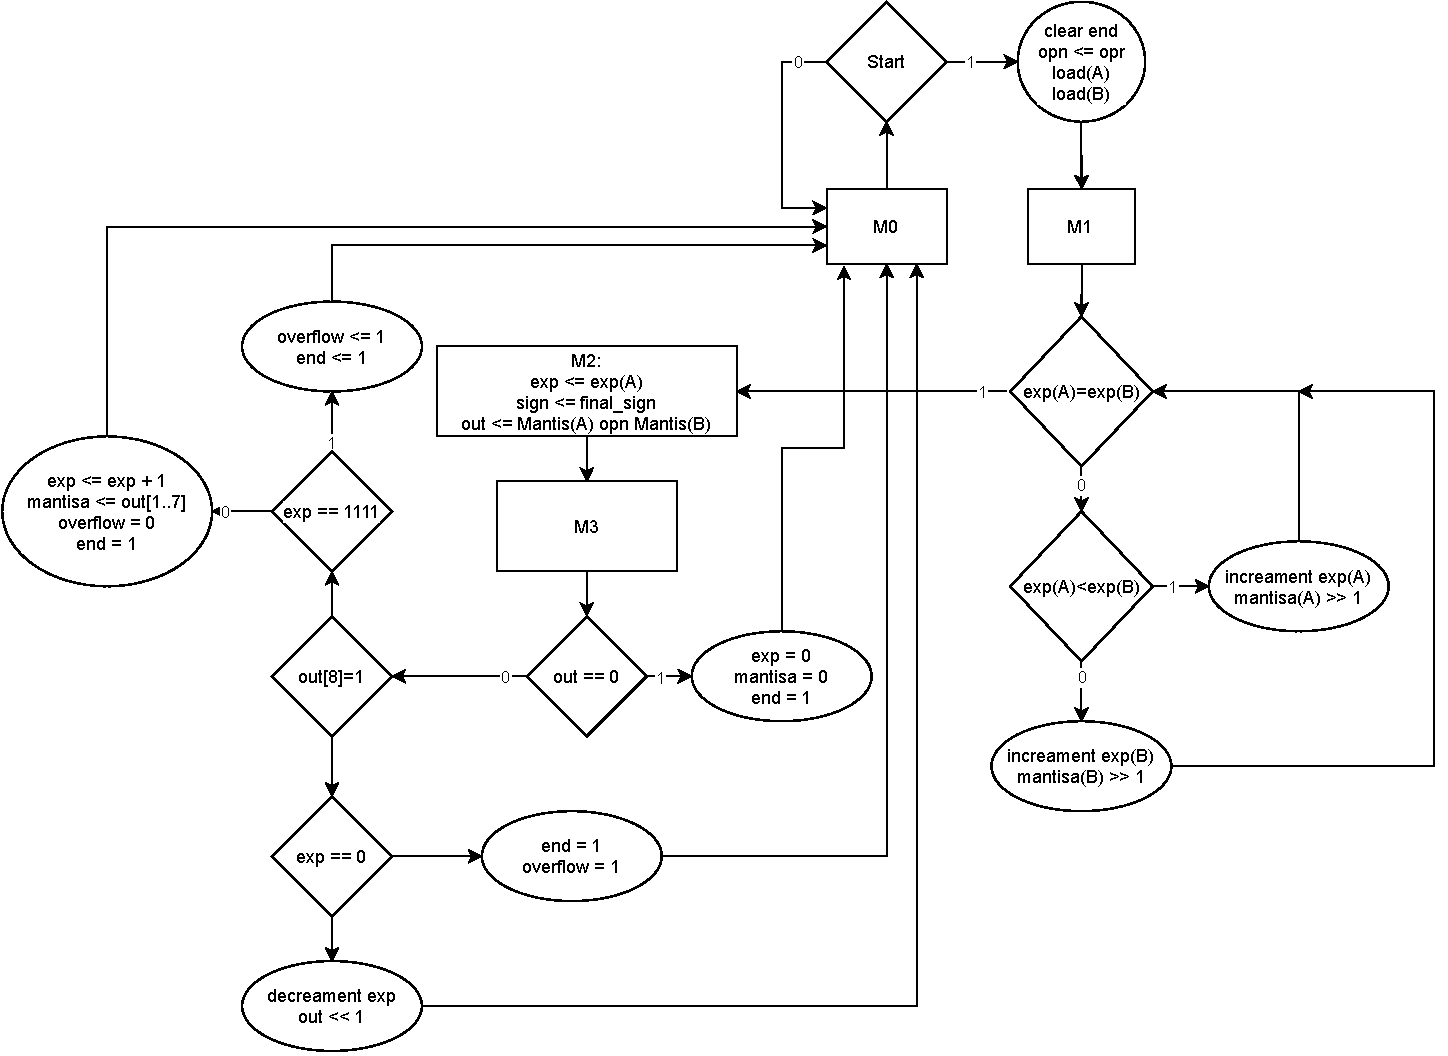
\includegraphics[scale=0.45]{./graphics/asm}
	\caption{\lr{ASM Chart}}
	\label{fig:asm}
\end{figure}

\subsection{مدار اصلی}
مدار اصلی کلاک، سیگنال شروع و ریست و عدد دهدهی را ورودی می‌گیرد. در خروجی هم سیگنال پایان و عدد دودویی وجود دارد. در شکل \ref{fig:outside} شمای کلی پیاده سازی آمده است. شکل \ref{fig:main} نیز مدار اصلی را نمایش می دهد.

\begin{figure}
	\centering
	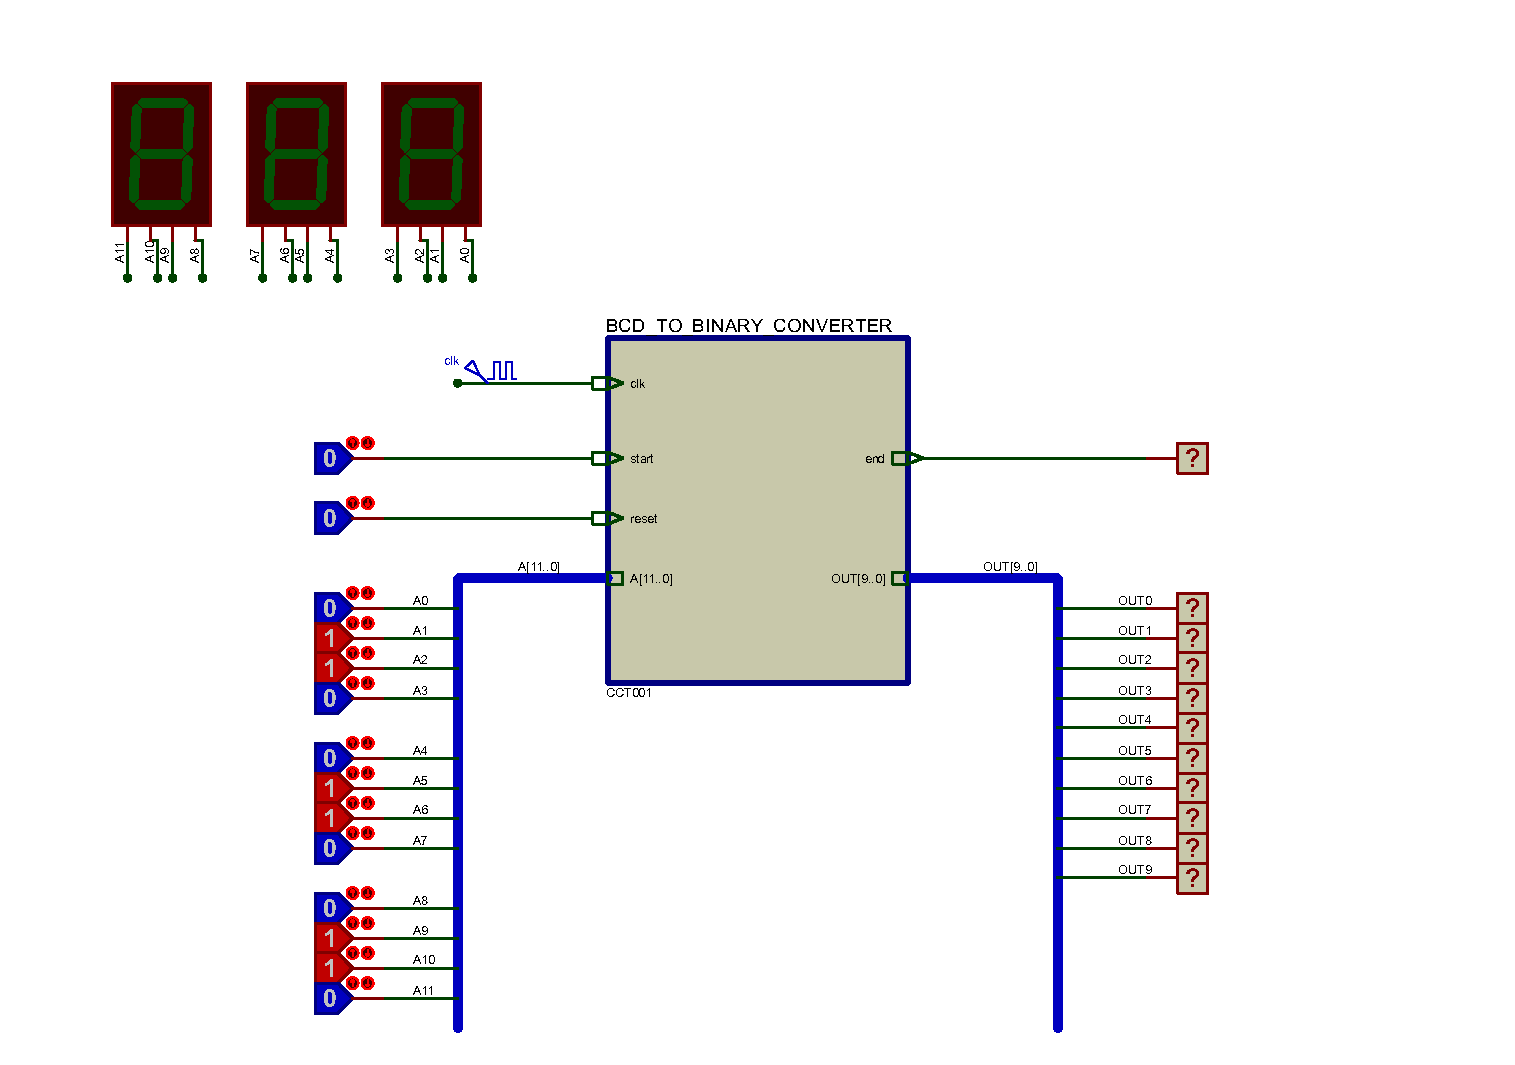
\includegraphics[scale=0.4]{./graphics/DecimalToBinaryConverter}
	\caption{شکل بیرونی مدار}
	\label{fig:outside}
\end{figure}

\begin{figure}
	\centering
	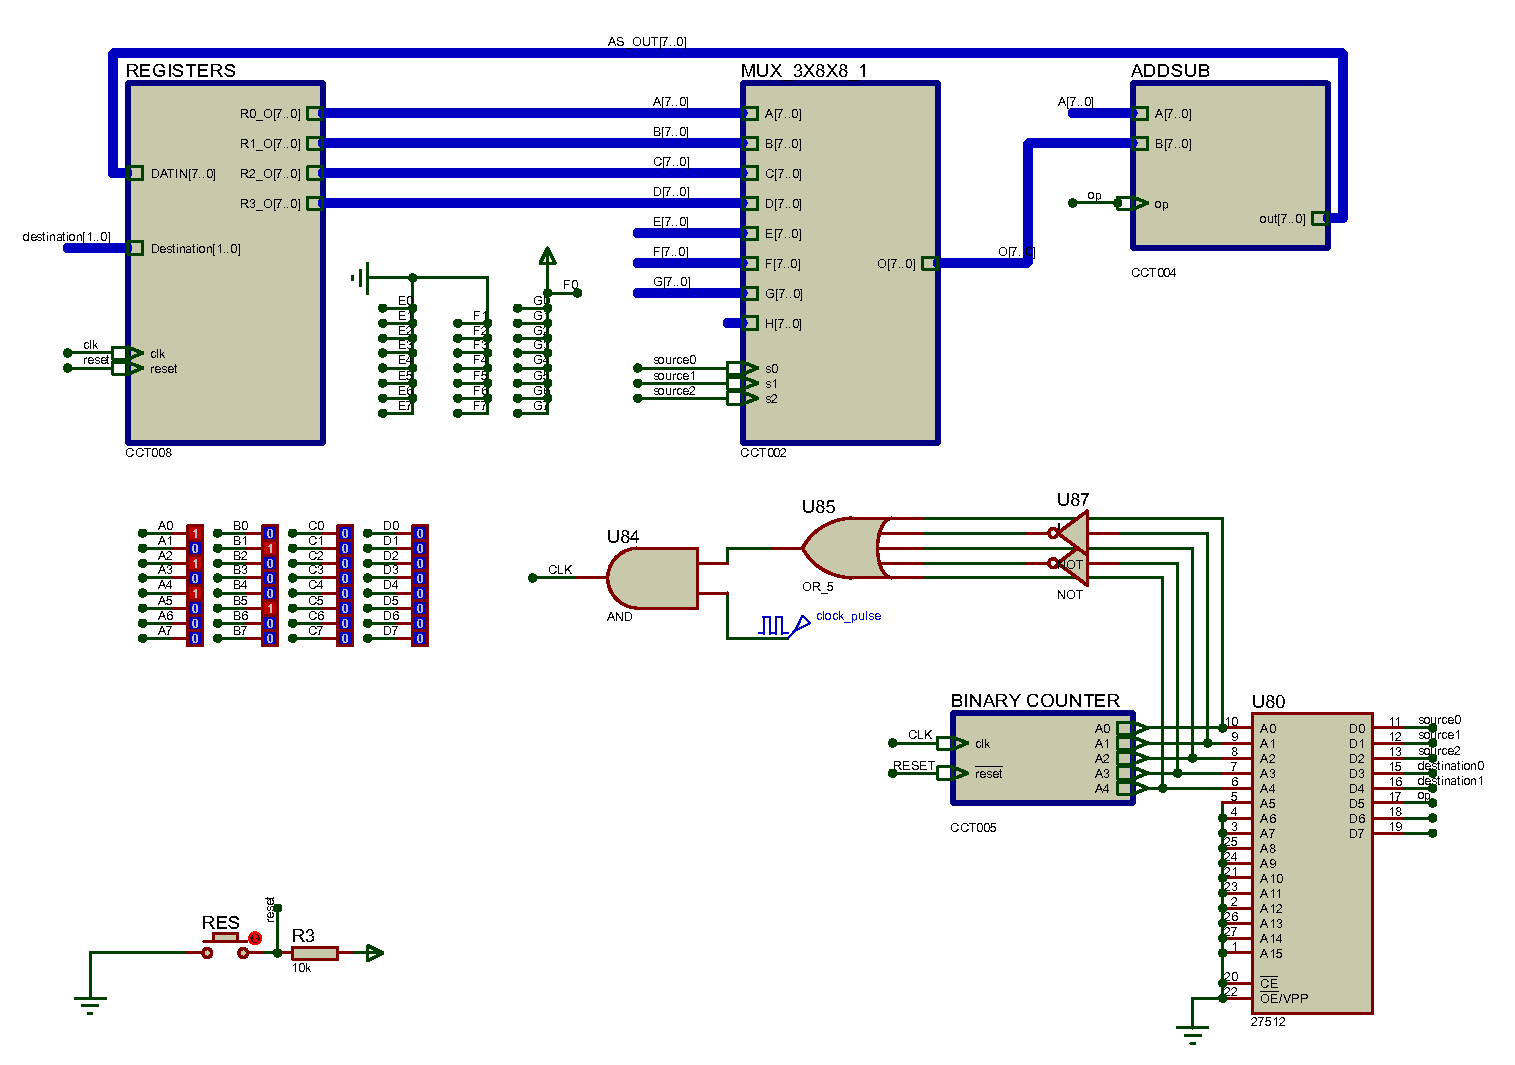
\includegraphics[scale=0.4]{./graphics/main}
	\caption{داخل مدار اصلی}
	\label{fig:main}
\end{figure}


\subsection{واحد کنترل}

بخش کنترلی مدار است که جابجایی بین استیت‌های مختلف را کنترل می‌کند. سیگنال شروع و ریست، حاصل \lr{Or} بیت‌های عدد دهدهی ورودی و سیگنال ده بودن شمارنده به همراه کلاک را ورودی می‌گیرد. در خروجی سه حالت اصلی مدار یعنی استیت‌های ابتدایی، شیفت و تفریق را نشان می‌دهد. شمای این بخش از مدار در شکل \ref{fig:cu} آمده است. روابط تبدیل حالات مدار به صورت زیر است:

\begin{align*}
	S_0^+ &= S_0 \cdot \texttt{\lr{Start}} + S_1 \cdot \overline{\texttt{\lr{DigitsOr}}} \cdot \texttt{\lr{CounterIsTen}}\\
	S_1^+ &= S_0 \cdot \overline{\texttt{\lr{Start}}} + S_1 \cdot \overline{\texttt{\lr{DigitsOr}}} \cdot \overline{\texttt{\lr{CounterIsTen}}} + S_2\\
	S_2^+ &= S_1 \cdot \overline{\texttt{\lr{DigitsOr}}}
\end{align*}

\begin{figure}
	\centering
	\includegraphics[scale=0.4]{./graphics/controlunit}
	\caption{واحد کنترل}
	\label{fig:cu}
\end{figure}

\subsection{سیگنال‌های کنترلی}

این بخش از مدار وظیفه تولید سیگنال‌های میانی با توجه به استیت فعلی مدار، عدد دهدهی و شمارنده را دارد. خروجی \verb!digits_or! درواقع \lr{Or} بیت‌های عدد دهدهی است که در استیت دوم استفاده می‌شود. \verb!counter_is_ten! نشان می‌دهد که شمارنده به 10 رسیده است یا خیر. با توجه به چارت زمانی که هنوز همه بیت‌های عدد دهدهی صفر نشده‌اند یا شمارنده به 10 نرسیده باشد و در استیت شیفت باشیم،   \verb!load_counter_shift_out! فعال است که نشان می‌دهد باید عدد دهدهی را یکی شیفت بدهیم و شمارنده را یک واحد افزایش بدهیم. خروجی \verb!mux_s! برای زمانی است که در استیت ابتدایی باشیم و سیگنال شروع بیاید (این سیگنال در بخش رجیسترها برای لود کردن ورودی اولیه در صورت صفر بودن و نگه‌داری ورودی قبلی درغیر این صورت است).
شمای این بخش در شکل \ref{fig:cs} آمده است.

\begin{figure}
	\centering
	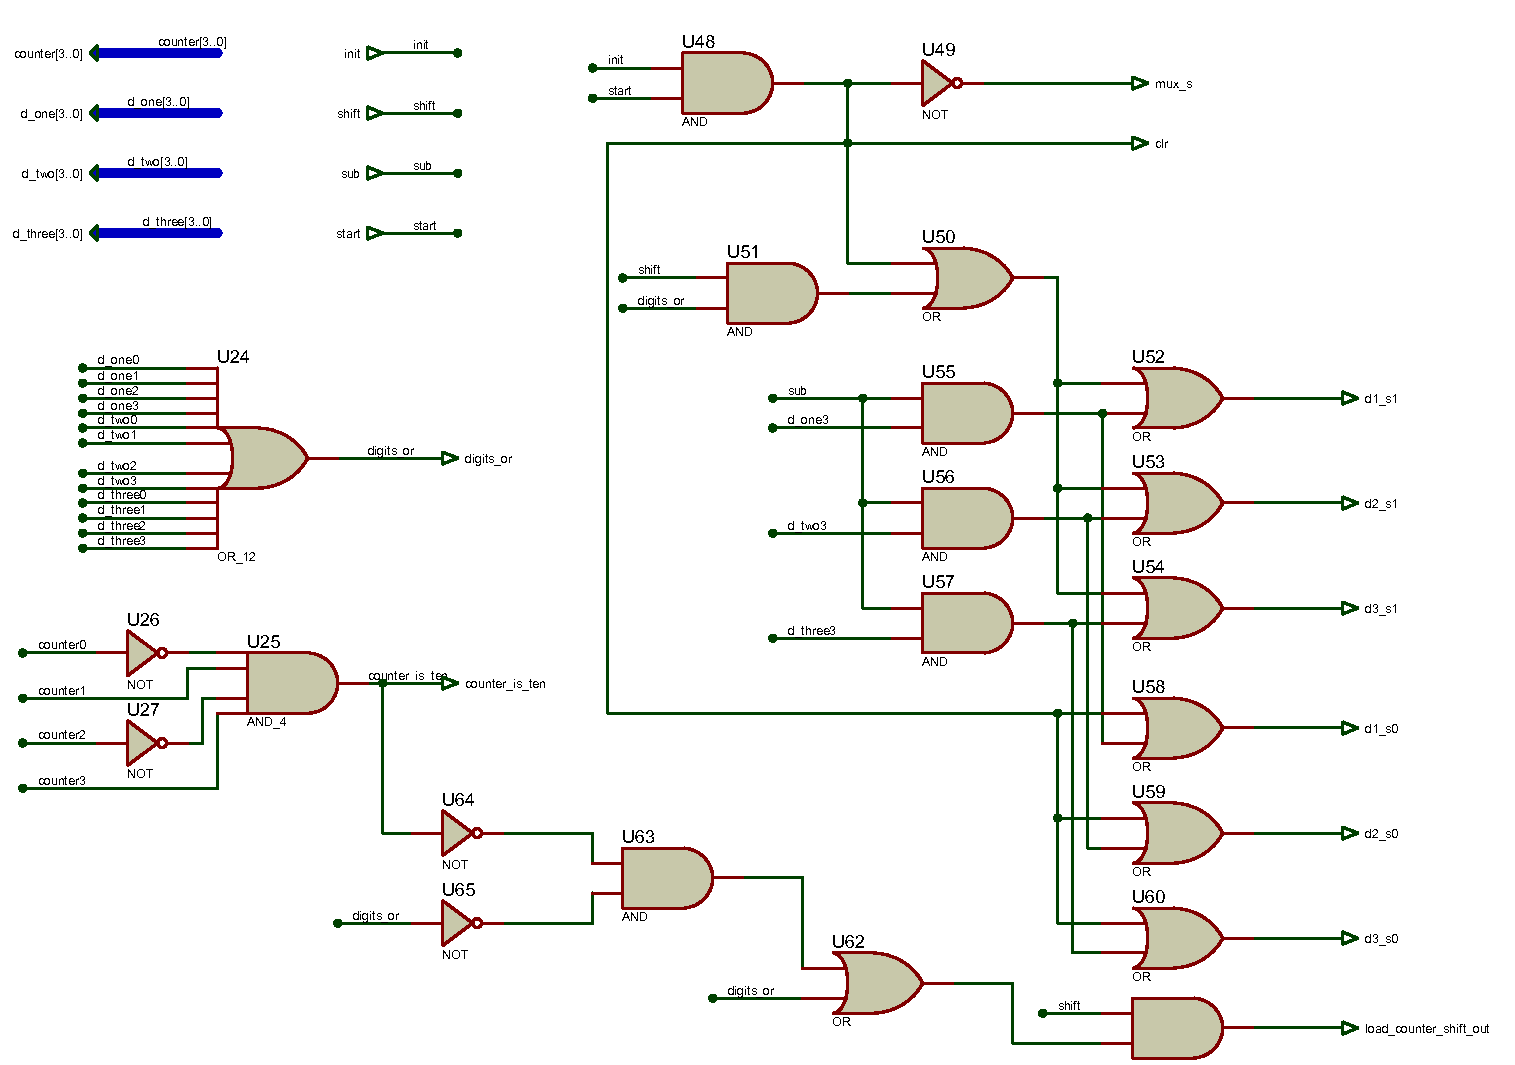
\includegraphics[scale=0.4]{./graphics/ControlSignals}
	\caption{سیگنال‌های کنترلی}
	\label{fig:cs}
\end{figure}

\subsection{رجیسترها}
این بخش از مدار با گرفتن ارقام عدد دهدهی ورودی آنها را در رجیستر ذخیره می‌کند. ماکس‌های دو به یک با توجه به \verb!mux_s! ورودی جدید را لود می‌کنند یا از ورودی قبلی استفاده می‌کنند. برای نگهداری ارقام از تراشه شیفت رجیستر ۴ بیتی 74194 استفاده شده است. از جمع کننده ۴ بیتی 4008 برای کم کردن 3 واحد از رقم درصورت نیاز استفاده شده است (ورودی \lr{A} آن رقم دلخواه و ورودی \lr{B} آن مکمل دو عدد 3 یعنی 1101 است). از دو شیفت رجیستر ۸ بیتی 74198 برای نگه‌داری عدد دودویی خروجی استفاده شده است. همچنین برای نگه‌داری شمارنده از تراشه 74194 استفاده شده که با اتصال به یک جمع‌کننده می‌تواند یکی‌یکی افزایش یابد.
شمای این بخش در شکل \ref{fig:reg} آمده است.

\begin{figure}
	\centering
	\includegraphics[scale=0.4]{./graphics/registers}
	\caption{رجیسترها}
	\label{fig:reg}
\end{figure}

\section{تست}
توجه کنید که برای تست مدار باید قبل از زدن سیگنال شروع یکبار آنرا ریست کرد.
شکل‌های \ref{fig:0} تا \ref{fig:962} مربوط به تست‌ اعداد تصادفی برای مدار هستند.

\begin{figure}
	\centering
	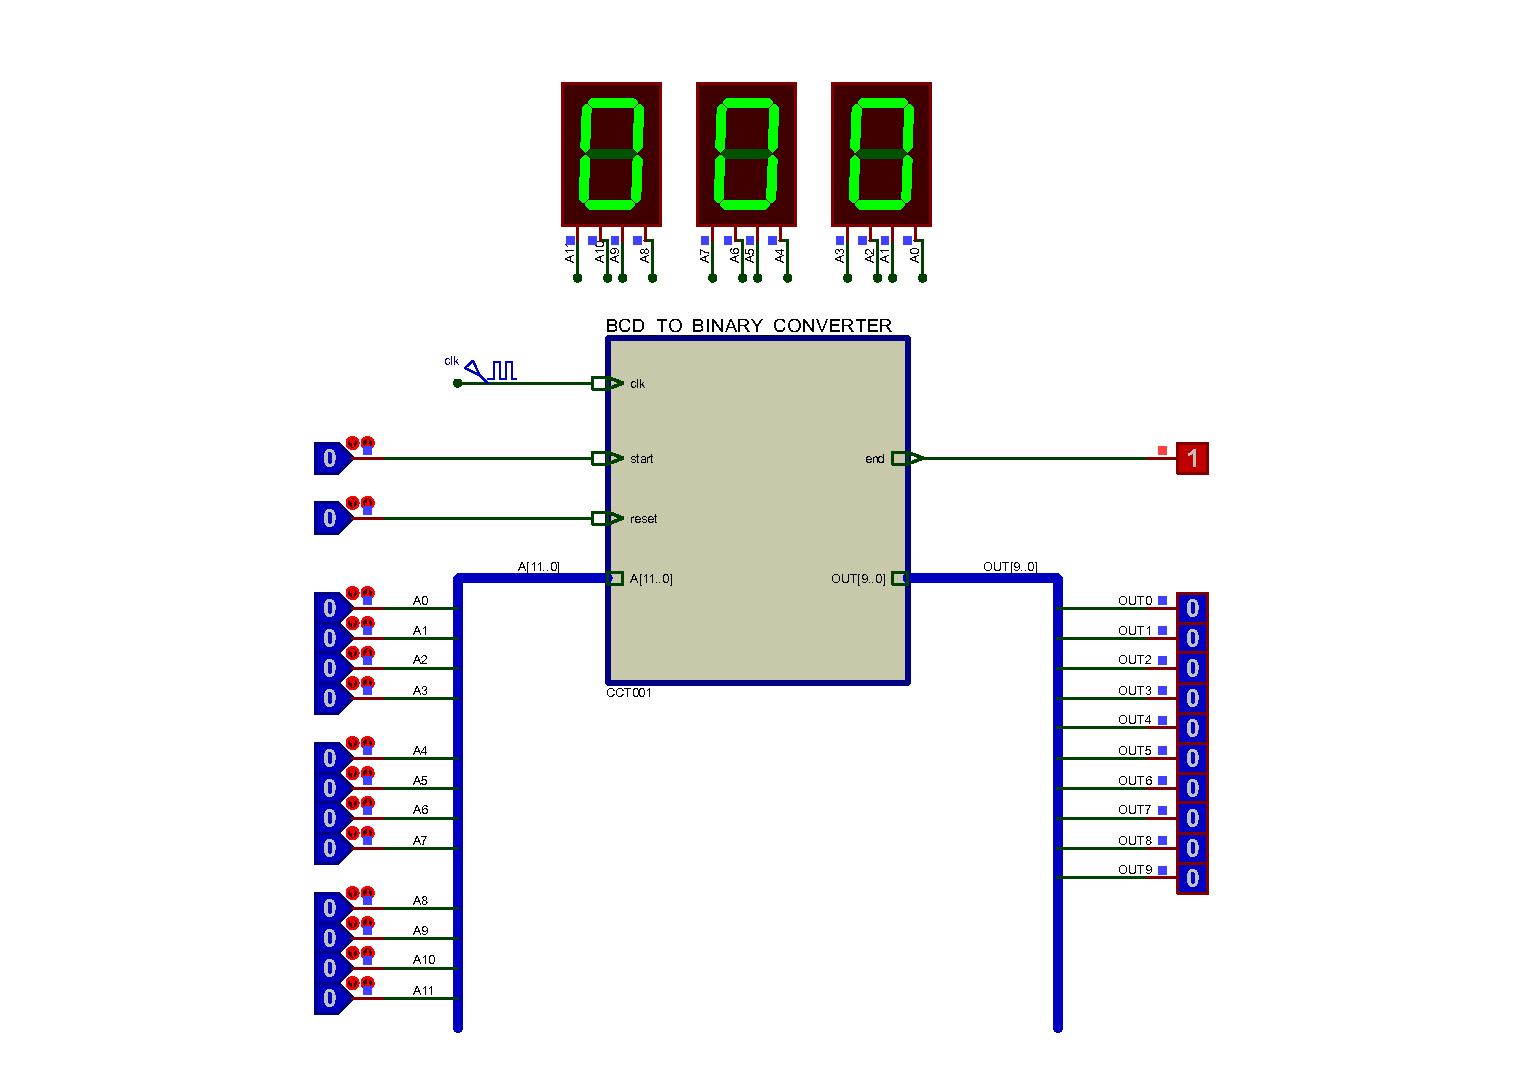
\includegraphics[scale=0.4]{./graphics/tests/0}
	\caption{تست عدد 0}
	\label{fig:0}
\end{figure}

\begin{figure}
	\centering
	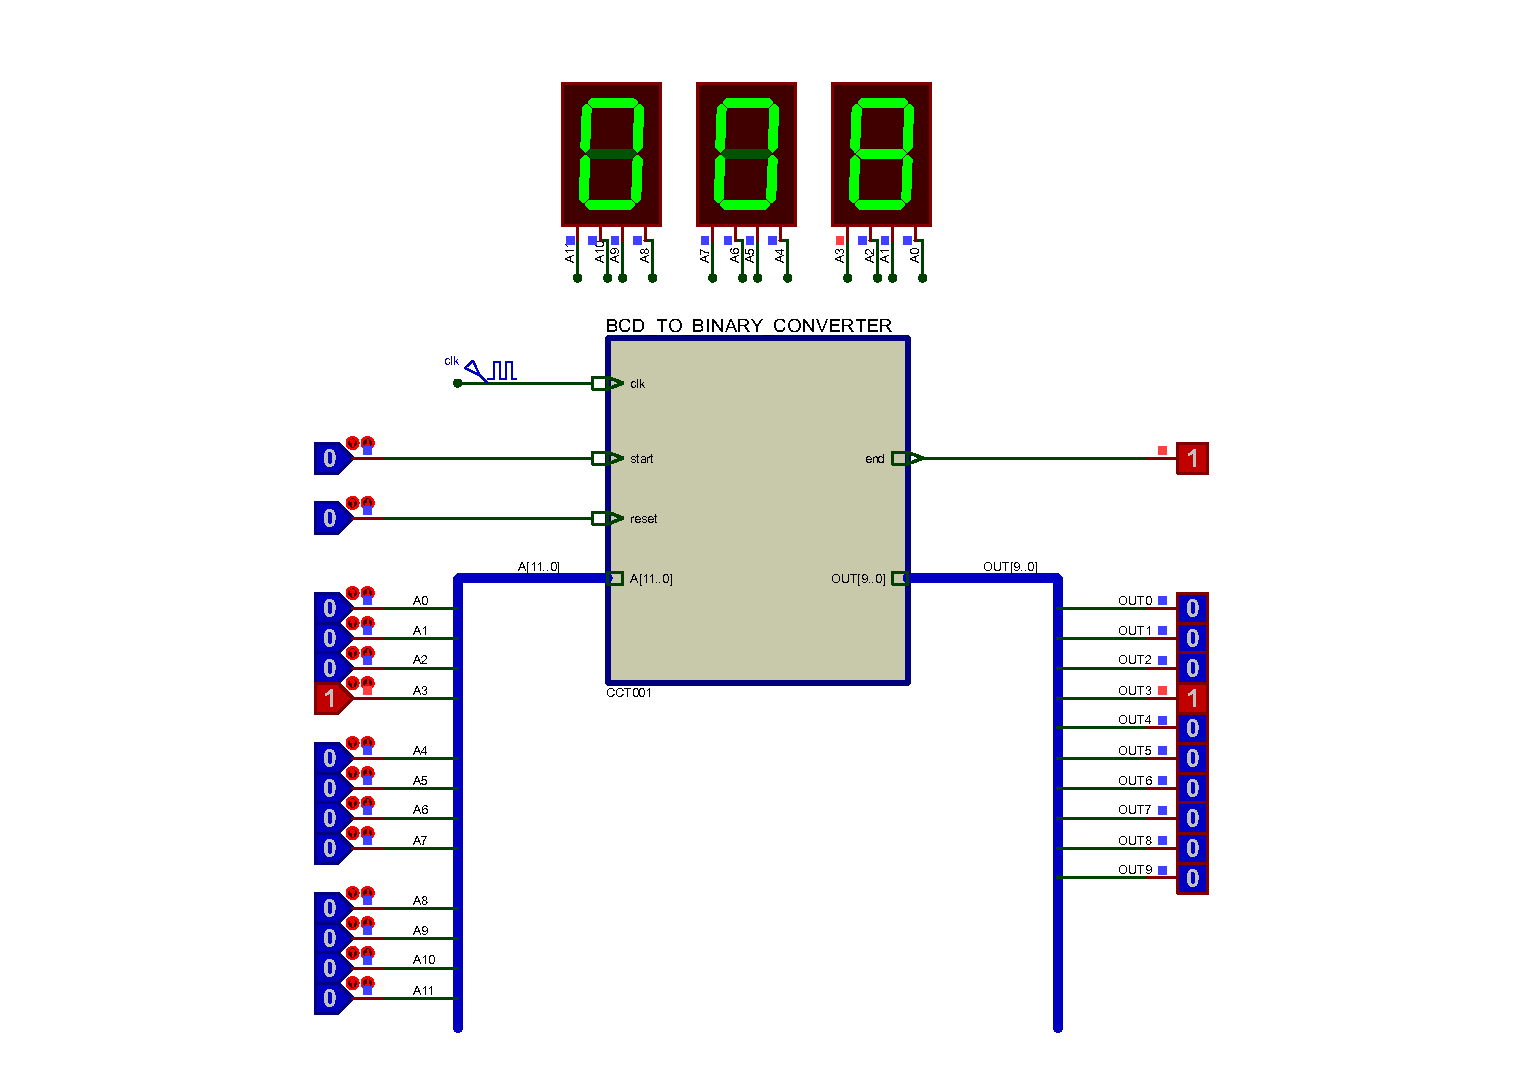
\includegraphics[scale=0.4]{./graphics/tests/8}
	\caption{تست عدد 8}
	\label{fig:8}
\end{figure}

\begin{figure}
	\centering
	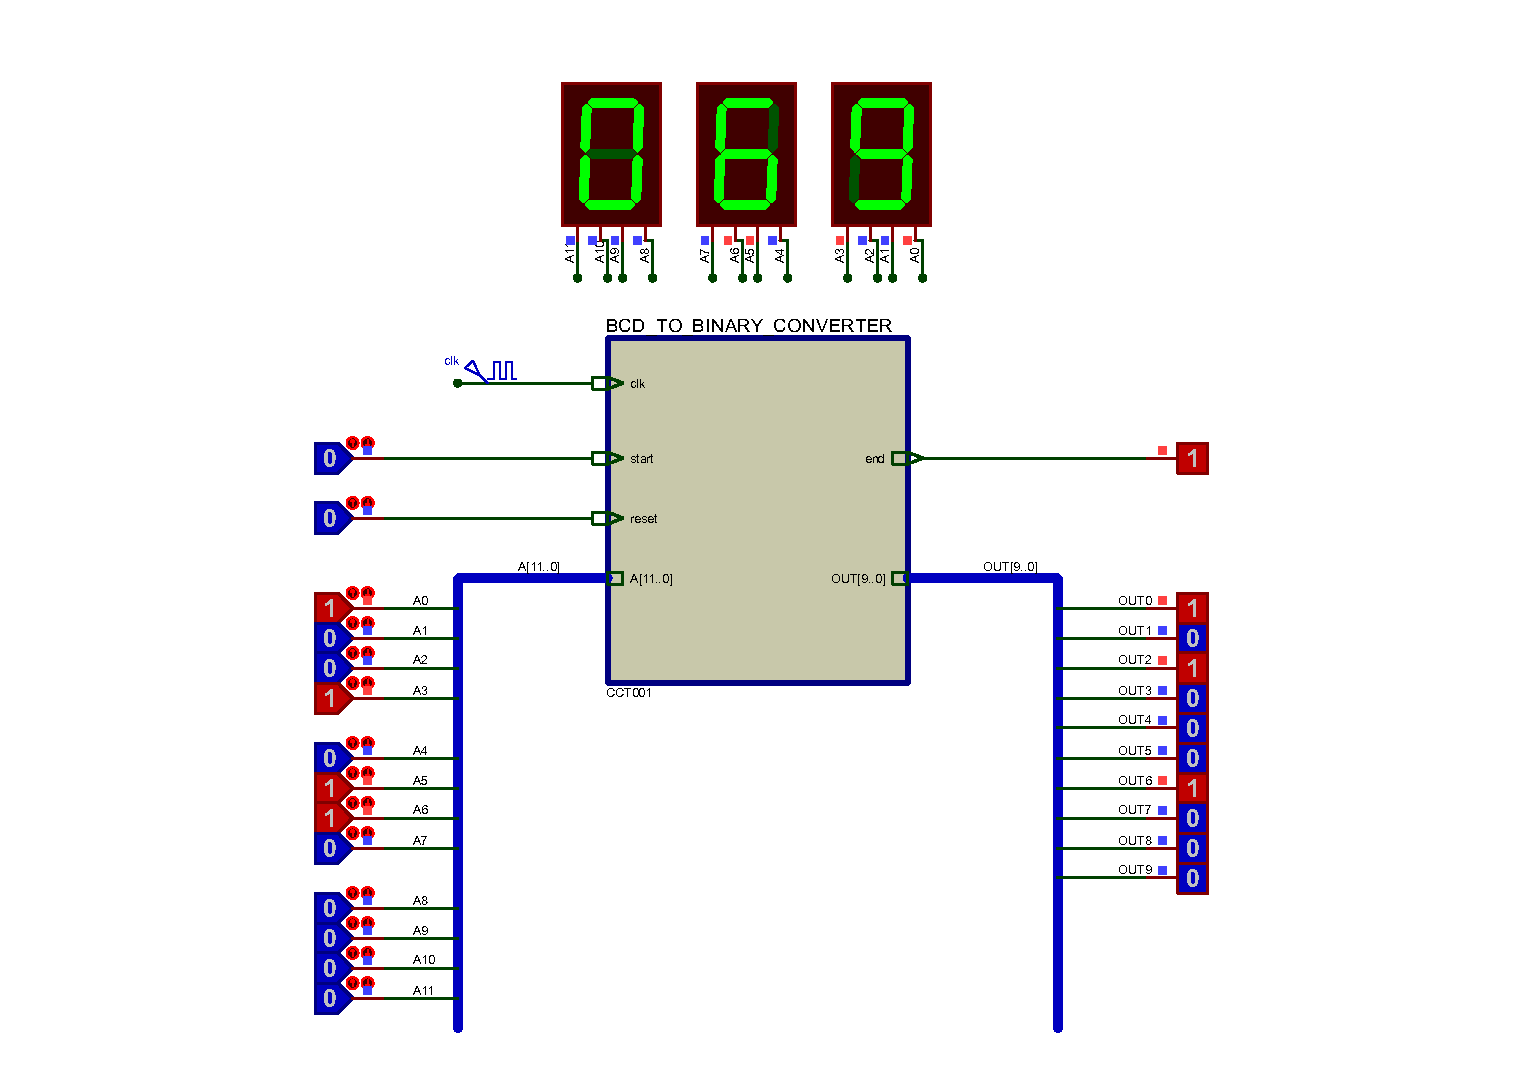
\includegraphics[scale=0.4]{./graphics/tests/69}
	\caption{تست عدد 69}
	\label{fig:69}
\end{figure}

\begin{figure}
	\centering
	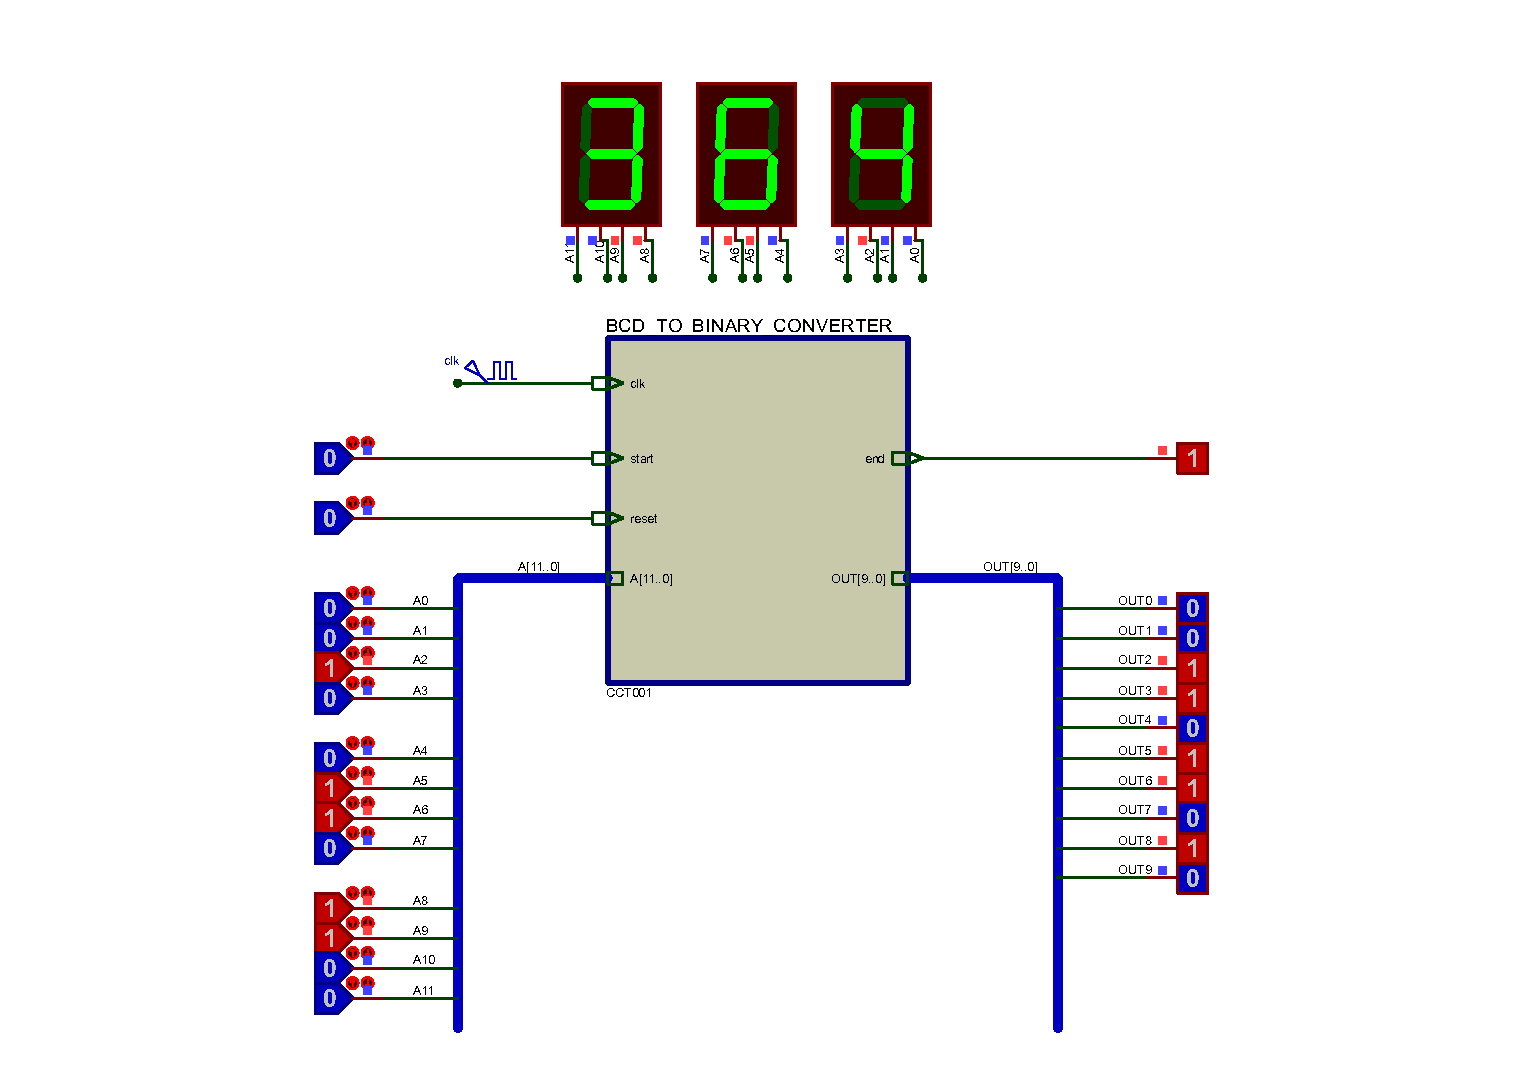
\includegraphics[scale=0.4]{./graphics/tests/364}
	\caption{تست عدد 364}
	\label{fig:364}
\end{figure}

\begin{figure}
	\centering
	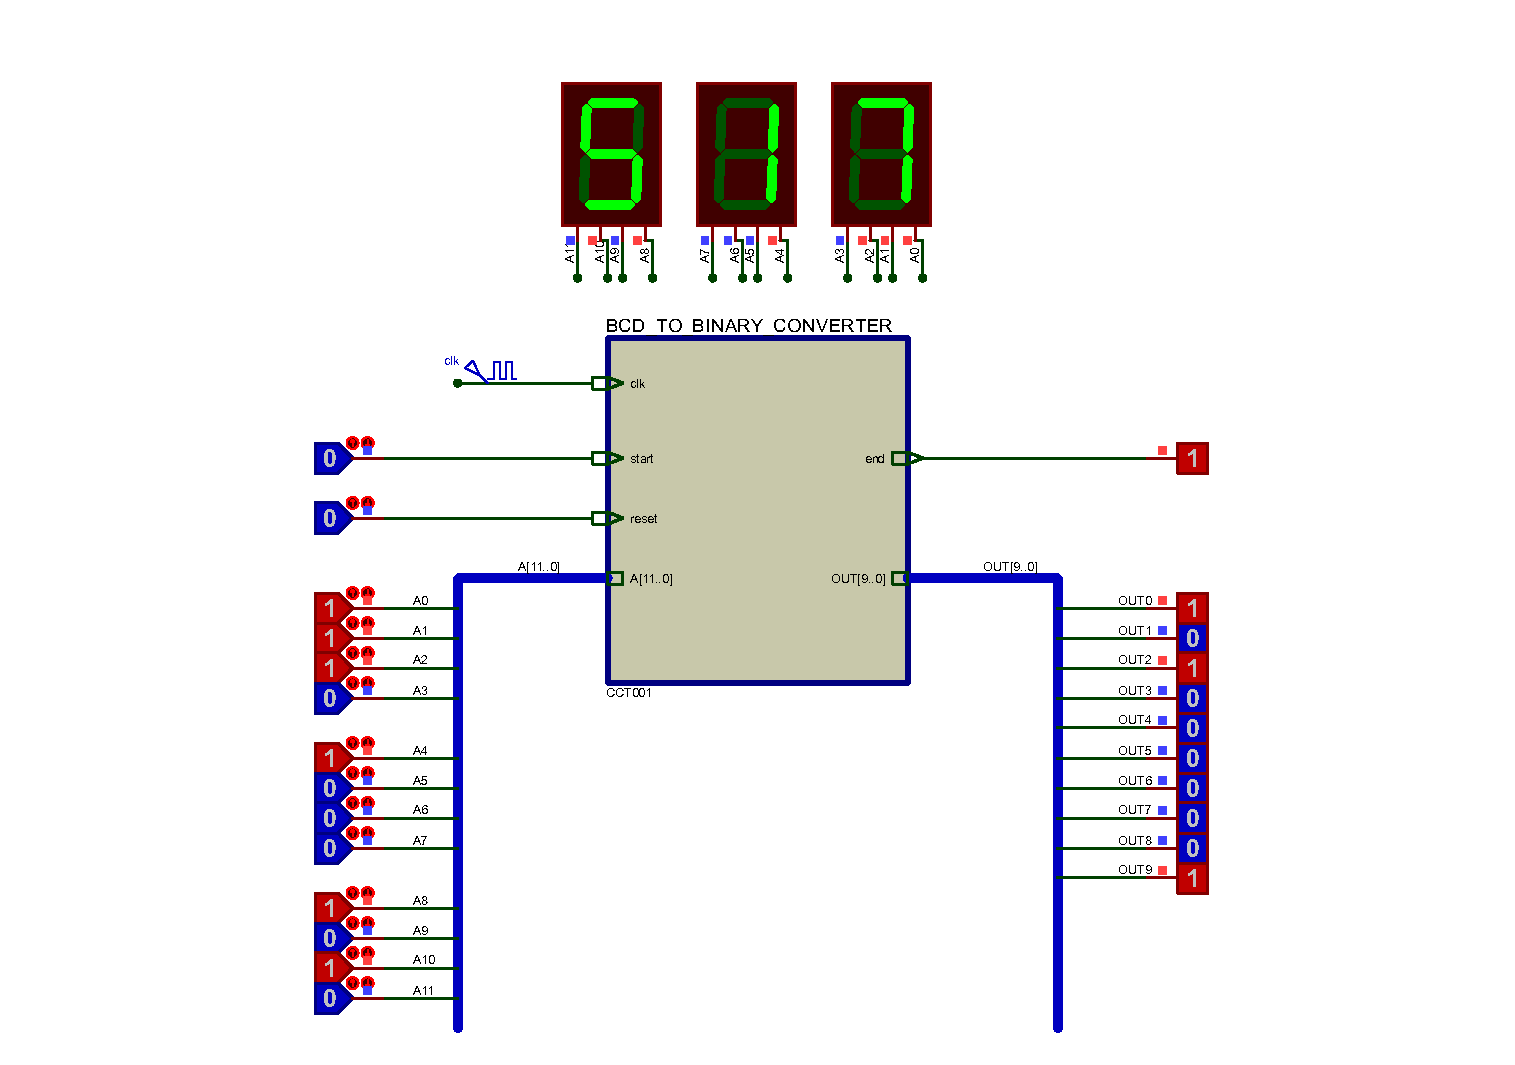
\includegraphics[scale=0.4]{./graphics/tests/517}
	\caption{تست عدد 517}
	\label{fig:517}
\end{figure}

\begin{figure}
	\centering
	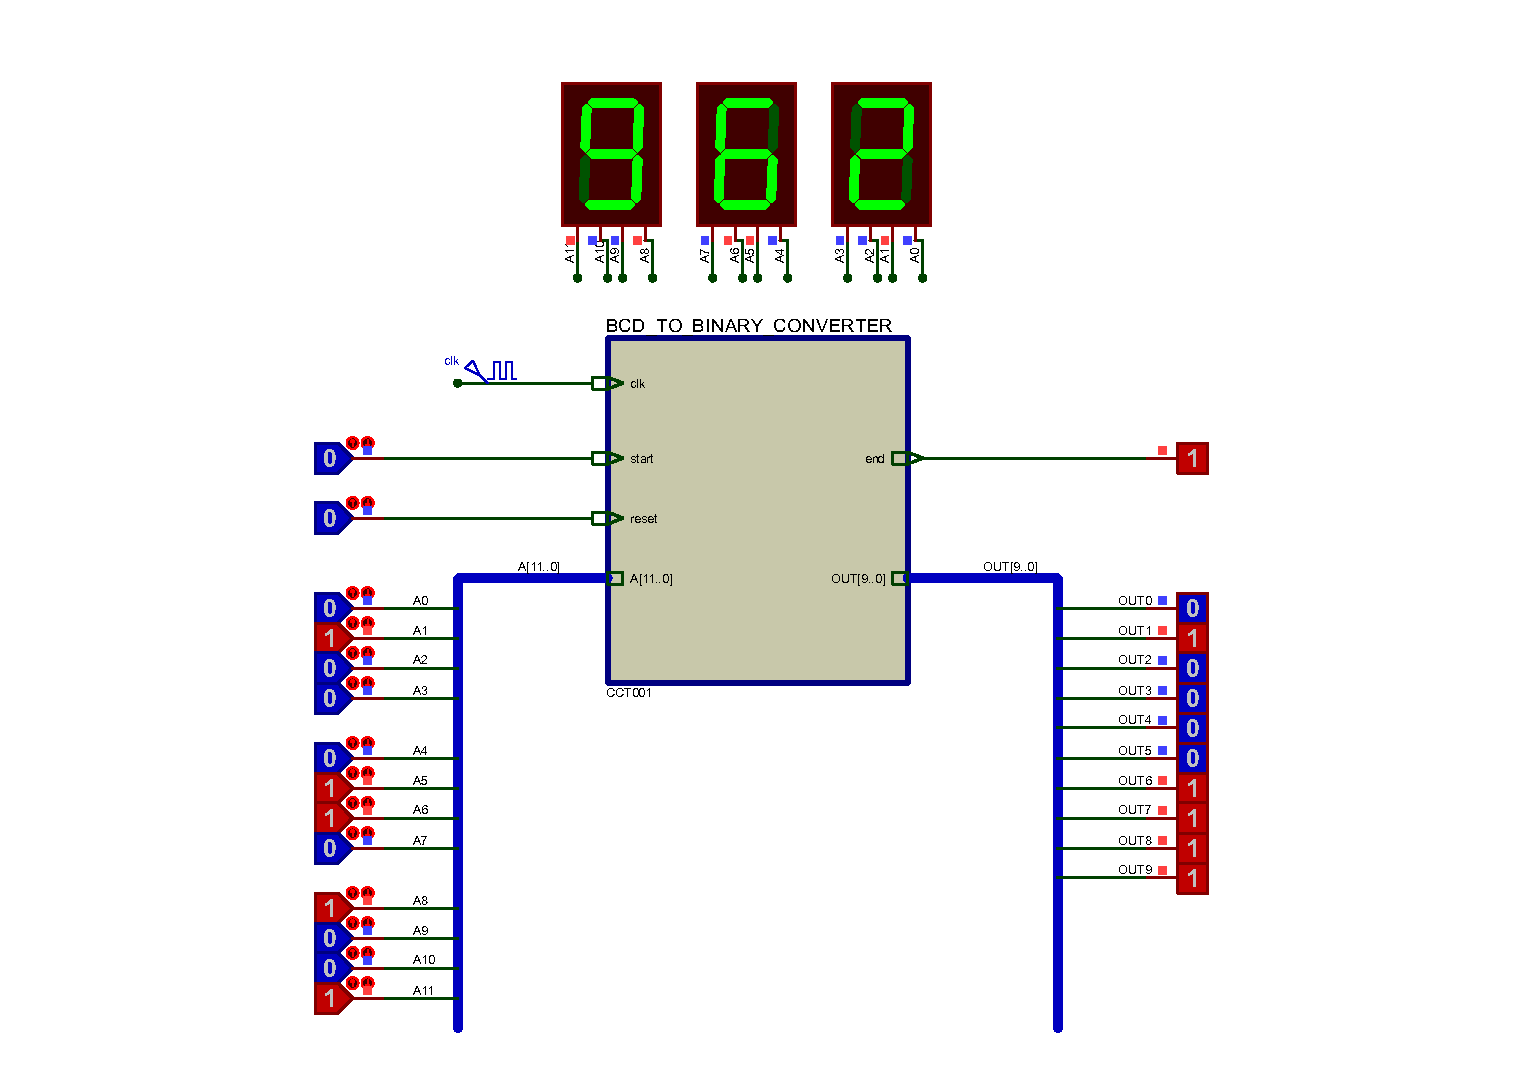
\includegraphics[scale=0.4]{./graphics/tests/962}
	\caption{تست عدد 962}
	\label{fig:962}
\end{figure}

\end{document}
